\documentclass[letterpaper,10pt]{article}

% Soporte para los acentos.
\usepackage[utf8]{inputenc}
\usepackage[T1]{fontenc}
% Idioma español.
\usepackage[spanish,mexico, es-tabla]{babel}
% Soporte de símbolos adicionales (matemáticas)
\usepackage{multirow}
\usepackage{amsmath}
\usepackage{amssymb}
\usepackage{amsthm}
\usepackage{amsfonts}
\usepackage{latexsym}
\usepackage{enumerate}
\usepackage{ragged2e}
\usepackage[hidelinks]{hyperref}
% Soporte para imágenes.
\usepackage{graphicx}
% Soporte para código.
\usepackage{listings}
% Soporte para URL.
\usepackage{hyperref}
\usepackage[all]{xy} %para diagramas conmutativos
% Modificamos los márgenes del documento.
\usepackage[lmargin=2cm,rmargin=2cm,top=2cm,bottom=2cm]{geometry}

\title{Computación Concurrente \\ Tarea 01}
\author{González Montiel Luis Fernando \\
312275136\\ }
\date{\today}

\begin{document}
\maketitle

\begin{enumerate}
    % Ejercicio 1.
    \item Considera el siguiente código que representa un contador:\\
Suponiendo que dos hilos se ejecutan concurrentemente sobre el mismo objeto de tipo Counter. Muestre la historia de una ejecución en la cual el resultado final del contador sea 10,8,5,1,0\\

    \textsc{Solución:}
	\\
	d) 1 \\Lo demostraremos por contradicción ya que sabemos que hay dos hilos h1, h2, entonces suponemos que el valor del contador termina en 1. Como sabemos que cada hilo ejecuta el metodo run en el cual la última instrucción es counter++, supongamos sin perdida de generalidad que el h2 termina la última ejecución de counter++, significa que el h2 leyó counter = 0, teniendo asi dos casos:\\
	Caso1. Es la última iteración del for en h2.\\
	Lo cual implica que h2 leyó 5 veces a counter = 0, lo cual no se podría puesto que h1 ha terminado con todas sus iteraciones y al menos aumento en una unidad el valor de counter, por lo tanto h2 no pudo haber leido counter = 0.\\
	Caso2. No es la última iteración del for en h2.\\
	Lo que significa que al menos h2 o h1 aumentaran en una unidad el valor de counter por lo que h2 no podría terminar leyendo en la penúlitma acción a counter = 0.\\
\\
	e) 0\\Como sabemos, hay dos hilos h1 y h2, para los cuales sin importar cuantas iteraciones tengan en sus ciclo for, la última instrucción que se lleva a cabo es counter++, por lo que al menos uno de los dos hilos h1 o h2, terminará su ejecución con esta instrucción y si en un inicio counter = 0, al final su valor será aumentado en una unidad. \\
	Por lo tanto el valor de counter no puede terminar con valor 0.\\
	
	
	
    % Ejercicio 2.
    \item Considera el siguiente código de un banco encargado de hacer una tranferencia:\\
    a) Demuestra que existe una condición de carrera.\\
	b) ¿Tiene una carrera por los datos?\\

    \textsc{Solución:}
         \\
    
	% Ejercicio 3.
    \item Considera un problema computacional que puede resolverse secuencialmente en tiempo $n^3$*$log_{10}$(n),con una unidad de tiempo de 2 nanosegundo ($10^{-9}$s). Des esta manera, si $n = 1000$, el cómputo tomaría $1000^{3}$*$log_{10}$(1000)*2ns = 6s. Supón que has creado un algoritmo concurrente que trabaja de manera completamente eficiente, es decir, el cómputo total tarda $\frac{n^3*log_{10}*n}{p}$ ($p$ es el número de hilos). Qué tan grande es la entrada que se puede manejar en:\\
    a) 1segundo, b) 1minuto, c) 1semana.\\
    Si tenemos los siguientes hilos disponibles:\\
    a) 8, b) 1000, c) 1,000,000\\

    \textsc{Solución:}
	\\
	\begin{itemize}
	
	\item[a, a) ] Un segundo y 8 hilos\\
	$$\frac{n^3*log_{10}*n*2x10^{-9}}{8}=1$$
	$$n = 1095.82$$
	
	\item[a, b) ] Un segundo y 1000 hilos
	$$\frac{n^3*log_{10}*n*2x10^{-9}}{1000}=1$$
	$$n = 5127.08$$
	
	\item[a, c) ] Un segundo y 1,000,000 hilos
	$$\frac{n^3*log_{10}*n*2x10^{-9}}{1000000}=1$$
	$$n = 47462.9$$
	
	\item[b, a) ] Un minuto y 8 hilos
	$$\frac{n^3*log_{10}*n*2x10^{-9}}{8}=60$$
	$$n = 4051.93$$
	
	\item[b, b) ] Un minuto y 1000 hilos
	$$\frac{n^3*log_{10}*n*2x10^{-9}}{1000}=60$$
	$$n = 19135.1$$
	
	\item[b, c) ] Un minuto y 1,000,000 hilos
	$$\frac{n^3*log_{10}*n*2x10^{-9}}{1000000}=60$$
	$$n = 178755$$
	
	\item[c, a) ] Una semana y 8 hilos
	$$\frac{n^3*log_{10}*n*2x10^{-9}}{8}=604800$$
	$$n = 79047.4$$
	
	\item[c, b) ] Una semana y 1000 hilos
	$$\frac{n^3*log_{10}*n*2x10^{-9}}{1000}=604800$$
	$$n = sin solución$$
	
	\item[c, b) ] Una semana y 1000000 hilos
	$$\frac{n^3*log_{10}*n*2x10^{-9}}{1000000}=604800$$
	$$n = sin solución$$
	
	\end{itemize}

    
	% Ejercicio 4.
    \item Da un ejemplo de un programa que:\\
	
    \textsc{Solución:}
	\\ 
	\begin{itemize}
	
	\item a) Tenga una condición de carrera y carrera por los datos.\\
	
	public run(int posicion)\\ 
	dato = genera();\\
	write(dato, posicion);\\
	\\
	Al no tener el synchronized los hilos pueden entrar en cualquier momento a la seccion critica, esto genera una condicion de carrera, cuando dos o más quieren modificar un dato en la base de datos, y al ponerle como paremetro la posicion mantemos la carrera con datos, ya que cada hilo va a modificar extactamente uno a uno esa posicion. \\
	\\
	\item b) Tenga una condición de carrera pero no carrera por los datos. \\
	
	public run() \\
	dato = genera();\\
	write(dato);\\
	\\
	Aquí lo que pasa es que la condición de carrera se da porque no los hilos no estan sincronizados y estos pueden entrar cuando quieran, y se quita la carrera de datos por el hecho de no especificar en qu parte de la base de datos se va a modificar, así que este puede acceder a modificar la linea dos veces.\\
	\\
	\item c) No tenga condición de carrera pero si carrera por los datos.\\
	
	public synchronized run(int posicion) \\
	dato = genera();\\
	write(dato, posicion);\\
	\\
	Cuando se ultilza el el synchronized, lo que pasa es que sincroniza los hilos uno a a vez para que cada uno tenga acceso a la seccion critia y pueda modificar los datos sin ningun problema, aparte con la posicion escribimos exactamente un dato a la vez. \\
	\\
	\item d) No tenga ni condición de carrera ni carrera por los datos.\\
	
	public synchronized run() \\
	dato = genera();\\
	write(dato);\\
	
	Al quitarle como parametro la posicion, no se sabe que parte se va a  modificar, al remover la posicion quitamos la carrera con dato, ya que esta puede acceder varias veces a la misma posicion, sin importar cual sea, puede acceder dos veces a la misma. \\
	
	\end{itemize}
	% Ejercicio 5.
    \item Calcula el speedup que tendría un programa con 100 procesadores si al medirlo en forma secuencial se tarda 188 segundos y con dos procesadores tarda 104 segundos.\\

    \textsc{Solución:}
	\\
	\begin{itemize}
	\item Observemos que usando la interpretacion de speedup de esta manera
	 $S(n)=\frac{T_{seq}}{T_{par}(n)}$
	tenemos que el speedup de dos procesadores en este ejemplo es:\\ 
	$S(2) = \frac{188s}{104s} \approx 1.8076$ y ahora ocupamos la formula del ejercicio anterior que es: 
	\begin{center}
	$s_{n}=\frac{s_{2}}{n(s_{2}-1)+s_{2}}$ \\
	\end{center}
	Ahora sustituimos en la formula por lo que obtenemos:\\
	$S(100) =\frac{1.8076}{100(1.8076-1)+1.8076}\approx 0.02189$ 
	\end{itemize}
	
	% Ejercicio 6.
    \item Usa la ley de Amdahl para resolver las siguientes preguntas:\\
    \textsc{Solución:}
	\\
	\begin{itemize}
	\item a) Supón que un programa tiene un método M que no puede ser paralelizado y que este método cuenta el 45\% del tiempo de la ejecución del programa. ¿Cuál es el límite de speedup general que se puede lograr ejecutando el programa en una máquina con n procesos?\\
	
	Respuesta:\\ Usando la ley de Amdahl $\frac{1}{(1-p)+\frac{p}{n}}$ tenemos lo siguiente $\frac{1}{(1-.45)+\frac{.45}{n}}$ a esto le aplicamos el limite de cuando n tiende a infinito lo cual la seccion $\frac{.45}{n} = 0$ sustituyendo tenemos $\frac{1}{.55} = 1.88x$ \\

	\item b) Supón que el método M cuenta el 35\% del tiempo de la ejecución del programa. Sea $s_{n}$ el speedup con n procesos. Tu jefe te dice que debes duplicar este speedup: la versión nueva del programa debe tener un speedup $s_{n}^{'} \geq 2 * s_{n}$. Tu buscas a un programador para reemplazar M con una version mejorada, k veces más rápida. ¿Qué valor de k es requerido?

	Respuesta:\\
	Observación 1:$s_{n} = \frac{1}{1-.65 +\frac{.65}{n}}$ donde aplicamos el limite donde n tiende a infinito tenemos como resultado $s_{n} = 2.85$ \\

	Observación 2:$s_{n}^{'} \geq 2*2.857$ que es lo mismo que $\frac{1}{p^{'}} \geq 5.7$ despejando a $p^{'}$ tenemos que debe tener valores entre $.824 \leq p^{'} < 1 $\\

	Usando las observaciones 1 y 2 tenemos que $s_{n}^{'} =  \frac{1}{(1-p)*k}$ donde k es la mejora del programa M sustituyendo tenemos que $5.68 = \frac{1}{(1-.65)*k}$ por lo tanto $K \approx.5030$\\
	
	\item c)Supón que el método M se puede acelerar tres veces. ¿Qué fracción de todo el tiempo de ejecución debe contar M para que se pueda doblar el speedup del programa?\\

	Respuesta:\\
	Sabemos que otra intepretacion del speedup es $t^{'} = \frac{t}{s}$ donde t es el tiempo a mejorar y s es la aceleracionmejorada y $t^{'}$ es el tiempo que debe tomar. Sustituyemdo en esta interpretacion tenemos que $t^{'} = \frac{3x}{2x} = \frac{3}{2}$ que es la fraccion de tiempo que se debe mejorar para doblar el speedup del programa M.
	
	\end{itemize}
	
	% Ejercicio 7.
    \item Tu amigo Juanito acaba de paralizar un código para su trabajo con la finalidad de que se ejecute más rápido. Por el momento, solo cuenta con una computadora con dos núcleos, la cual produjo un speedup $S_{2}$. Juanito quiere saber cuántos nucleos adicionales tendría que comprar para alcanzar el mejor desempeño sin desperdiciar recursos.\\
    
    Ayuda a tu amigo y utiliza la Ley de Amdahl para derivarle una fórmula $S_{n}$ (speedup con n procesadores) en términos de n y $S_{2}$.\\
    
    Supongamos que vuelves a encontrar a Juanito y te dice logró optimizar su programa 10x haciendo únicamente el 35\% de su código paralelo. ¿Lo que dice es verdad? Justifica tu respuesta.\\
	
    \textsc{Solución:}
	\\
	
	% Ejercicio 8.
    \item Propón un algoritmo de exclusión mutua para 3 hilos basado en turnos round robin.\\
    \textsc{Solución:}
	\\
	Propuesta.\\
	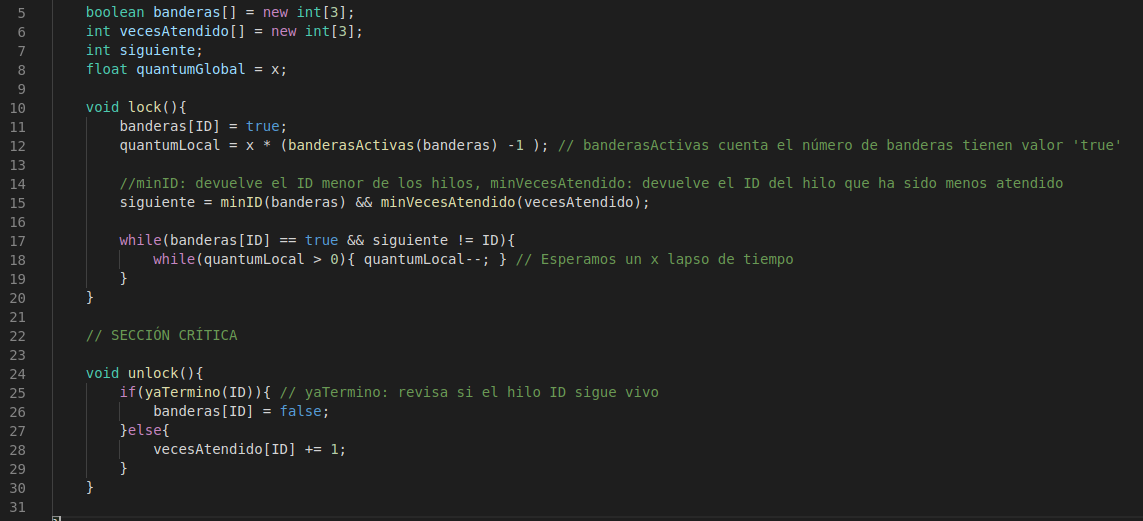
\includegraphics[width=\textwidth]{EM.png}\\ 
	\begin{itemize}
	\item[a) ] Demuestra que cumple con la propiedad de exclusión.
	[Por Contradicción.]

	Sean A, B y C, supongamos que el valor de ID es menor consecuentemente.
	Supongamos que existe una ejecución $CS_A \nrightarrow CS_B$ y $CS_B \nrightarrow CS_A$.
	para cualesquiera dos procesos. Tenemos dos casos dado el algoritmo para que esto suceda:
	\begin{itemize}
	\item[Caso a. ] Tienene diferente cantidad de veces atendidos. Supongamos que A ha sido atendido menos veces.\\
	Primero ocurrió que:
	\[1a)write_A(banderas[A] = true)\] \[ \rightarrow write_A(siguiente = (minID\hspace{0.2cm}AND \hspace{0.2cm}minVecesAtendido) = A)\]
	Para que A entre a la sección crítica:
	\[1b) read_A(banderas[A] == true)\hspace{0.2cm}AND\hspace{0.2cm}read_A(siguiente == A) \rightarrow CS_A\]
	Además, primero ocurrió que:
	\[2a)write_B(banderas[B] = true)\] \[ \rightarrow write_B(siguiente = (minID\hspace{0.2cm}AND \hspace{0.2cm}minVecesAtendido) = A)\]
	Para que B entre a la sección crítica:
	\[2b) read_B(banderas[B] == true)\hspace{0.2cm}AND\hspace{0.2cm}read_B(siguiente == B) \rightarrow CS_B\]
	Por lo que hay una contradicción entre 2a y 2b ya que la varibale "siguiente" fue escrita con el valor de "A" pero B leyó que el siguiente era "B"

	\item[Caso b. ] Tienen la misma cantidad de veces atendidos.\\

	De manera análoga al caso anterior, suponiendo las misma condiciones. El valor que leería B en la variable "siguiente" es "B" para entrar en sus sección crítica, pero por el valor léxcio de A, es menor que B (o C), por lo que la varibale A sería escrita con el valor de "A" y de esta manera B no podría leer "B" si en la última escritura de "siguiente" fue "A".

	\end{itemize} 
	\item[b) ] ¿Es libre de deadlock?\\

	Sí, ya que por el valor que se necesita para dejar de estar bloqueado, es del valor de los ID de cada hilo, estos ID's son únicos y en algún momento pasará debido a que se van atendiendo a los procesos según su cantidad de veces que se antendieron y el valor de su ID, por lo que no importa si tienen el mismo valor en atenciones se desempatará por el valor de su ID que es único.

	\item[c) ] ¿Es libre de hambruna?\\

	Sí ya que como es con base en un 'quantum' especificado, cada uno irá siendo atendido en determinado tiempo, y junto con su atención de cada proceso según el valor de su ID, estos irán siendo atendidos al menos en una ocasión.

	\end{itemize}	
	
	
	% Ejercicio 9.
    \item Menciona al menos 2 ventajas de usar hilos heredando de la clase Thread y dos ventajas de implementar la interfaz Runnable. ¿En qué casos usarías qué forma?\\

    \textsc{Solución:}
	\\
	Una ventaja de que si una clase define un hilo que implementa la interfaz Runnable, tiene la posibilidad de extender una clase, ya que en Java, la herencia múltiple no está permitida, por lo tanto, después de que una clase extiende la clase Thread, no puede extender ninguna otra clase.\\
	Otra ventaja sería que como varios subprocesos comparten el mismo objeto, se utiliza menos memoria, a diferencia de la clase Thread, que cada hilo crea un objeto único y se asocia con él, entonces a medida que cada hilo crea un objeto único, se requiere más memoria.\\
	
	Por otro lado unas ventajadas de hilos heredados de la clase Thread es que extender una clase generalmente significa agregar nuevas funcionalidades, modificar o mejorar comportamientos.
	Y otra ventaja es que la clase Thread extensible introduce un acoplamiento estrecho ya que la clase contiene el código de la clase Thread y también el trabajo asignado al hilo.\\
	
	
	% Ejercicio 10.
    \item Tu eres uno de los P prisioneros recién arrestados durante una manifestación en pro de las ciencias de la computación. El guardia, un computólogo transtornado, hace el siguiente anuncio:\\
   
    Escuchenme bien porque no lo repetiré. Hoy por la noche podrán juntarse y
planear una estrategia, pero después de hoy, cada uno estará en celdas aisladas y no tendrán comunicación con nadie. He puesto un cuarto con un apagador, el cual puede estar en un estado de prendido o apagado, sin embargo, no está conectado a nada.\\
De vez en cuando, seleccionaré a un prisionero aleatoriamente para entrar al cuarto con el apagador. Ese prisionero podría cambiar el estado del apagador, de prendido a apagado o viceversa, o podría dejarlo tal y como lo encuentró\\
Me aseguraré que para cualquier P, eventualmente cada uno de ustedes visitará el cuarto al menos N veces pero sin ningún orden en particular. Cuando ustedes lo deseen, podrían declarar la siguiente frase: “todos hemos visitado el cuarto con el apagador al menos una vez”. Si su afirmación es correcta, ¡los liberaré!, de lo contrario serán comida de cocodrilos. Escojan sabiamente y que comience el juego.\\

	\begin{itemize}
	\item a) Desarrolla una estrategia ganadora para cuando sabes que el estado inicial del apagador comienza en apagado.
	
	\item b) Desarrolla una estrategia ganadora para cuando no sabes el estado inicial del apagador
	\end{itemize}

    \textsc{Solución:}
	\\
	\\
	
	
	Referencias:\\
	\url{https://es.fondoperlaterra.org/comdifference-between-thread-class-and-runnable-interface-in-java-53#:~:text=La%20diferencia%20b%C3%A1sica%20entre%20Thread,Runnable%20comparte%20el%20mismo%20objeto.}
	
	\url{https://es.stackoverflow.com/questions/38201/diferencia-entre-runnable-handler-thread}
    

	
 \end{enumerate}



\end{document}
